\documentclass[11pt]{elegantbook}

\title{Polynôme} % 这里放置书名
% \subtitle{Subtitle} % 这里放置副标题

\author{CatMono} % 这里放置作者名
\date{September, 2025} % 这里放置日期
\version{0.1} % 这里放置版本号
% \institute{Elegant\LaTeX{} Program} % 这里放置机构名
% \bioinfo{Custom Key}{Custom Value} % 这里放置自定义信息

% \extrainfo{extra information} % 这里放置额外信息,将显示在最下方中央

\setcounter{tocdepth}{2} % 设置目录深度
\setcounter{secnumdepth}{2} % 设置章节编号深度


% \logo{logo-blue.png} % 这里放置封面logo,默认从figure目录下寻找
% \cover{LogiqueMathematique.png} % 这里放置封面图片,默认从figure目录下寻找

% modify the color in the middle of titlepage
\definecolor{customcolor}{RGB}{32,178,170} % 自定义颜色
\colorlet{coverlinecolor}{customcolor}
\usepackage{cprotect} % 保护命令参数不被 LaTeX 解析器过早处理,允许在某些特殊环境中使用脆弱命令(fragile commands)。
\usepackage{xeCJK} % 使用 xeCJK 包支持中文


% ===== 开始文档 =====
\begin{document}

\maketitle %生成文档的标题页,根据之前定义的标题信息(如标题、作者、日期等)自动创建一个格式化的标题页

% === 前言部分 ===
\frontmatter        % 开始前言,页码为 i, ii, iii...
\tableofcontents    % 目录 (页码: i, ii)
% \listoffigures      % 图表目录 (页码: iii)
% \listoftables       % 表格目录 (页码: iv)

\chapter{Preface}   % 前言章节(无编号,页码: v, vi...)
This is the preface of the book...

% \chapter{Acknowledgments}  % 致谢(无编号)
% I would like to thank...
% === 正文部分 ===
\mainmatter         % 开始正文,页码从 1 重新开始

\chapter{Preliminaries} % 这里放置章节标题


\chapter{Univariate Polynomial Ring}
\section{Univariate Polynomials}

\section{Division}

\begin{theorem}{Euclidean Division (Division with Remainder)}
    Let \( f(x), g(x) \in P[x] \) with \( g(x) \neq 0 \). 
    Then there exist unique polynomials \( q(x), r(x) \in P[x] \) such that
    \[
    f(x) = g(x) \cdot q(x) + r(x)
    \]
    where \( r(x) = 0 \) or \( \deg(r) < \deg(g) \).
\end{theorem}

\begin{definition}{Exact Division}
    If there exists \( h(x)\in P[x] \) such that \( f(x) = g(x) \cdot h(x) \), 
    we say that \( g(x) \) divides \( f(x) \) and write \( g(x) \mid f(x) \).
    (In other words, the remainder \( r(x) = 0 \).)
\end{definition}

\begin{property}
    
\end{property}

\begin{caution}
    In Euclidean division, \( g(x) \neq 0 \) is required. 
    However, in the case of \( g(x) \mid f(x) \), \( g(x) \) can equal \( 0 \). 
    In this situation, \( f(x) = g(x)h(x) = 0 \cdot g(x) = 0 \), 
    meaning that the \textbf{zero polynomial can only divide the zero polynomial}.
\end{caution}

\section{Greatest Common Divisor and Relatively Prime}
\begin{leftbarTitle}{Greatest Common Divisor}\end{leftbarTitle}
\begin{definition}{Greatest Common Divisor (GCD)}
    Let \( f(x), g(x) \in P[x] \). 
    A polynomial \( d(x) \in P[x] \) is called a greatest common divisor of \( f(x) \) and \( g(x) \) if:
    \begin{enumerate}
        \item \( d(x) \mid f(x) \) and \( d(x) \mid g(x) \);
        \item For any polynomial \( h(x) \in P[x] \), 
            if \( h(x) \mid f(x) \) and \( h(x) \mid g(x) \), then \( h(x) \mid d(x) \).
    \end{enumerate}
    The greatest common divisor of \( f(x) \) and \( g(x) \), 
    whose leading coefficient is \(1\) (also called \textbf{monic}), is denoted as \( \left(f(x), g(x)\right) \).
\end{definition}

\begin{property}
    
\end{property}

\begin{theorem}{Euclidean Algorithm}
    For all \( f(x), g(x) \in P[x] \), there exists \( d(x) \in P[x] \), 
    where \( d(x) \) is a greatest common divisor of \( f(x) \) and \( g(x) \), 
    and \( d(x) \) can be expressed as a linear combination of \( f(x) \) and \( g(x) \), 
    i.e., there exist \( u(x), v(x) \in P[x] \) such that
    \[
    d(x) = u(x)f(x) + v(x)g(x).
    \]
    The converse proposition does not hold in general.
\end{theorem}



\begin{leftbarTitle}{Relatively Prime}\end{leftbarTitle}

\begin{definition}{Relatively Prime}
    Two polynomials \( f(x) \) and \( g(x) \) in \( P[x] \) are called relatively prime 
    if \( (f(x), g(x)) = 1 \), 
    meaning they have no common divisor other than the zero-degree polynomial (nonzero constant).
\end{definition}

\section{Least Common Multiple}


\chapter{Factorization and Roots}

\section{Irreducible Polynomials}
\begin{definition}{Irreducible Polynomial}
    A polynomial \( p(x) \) of degree \( \geq 1 \) over a field \( P \) 
    is called an irreducible polynomial over the field \( P \) 
    if it cannot be expressed as the product of two polynomials of 
    lower degree than \( p(x) \) over the field \( P \).
\end{definition}

\begin{proposition}
    For all \(f(x), g(x)\in P[x]\), \(p(x)\) is an irreducible polynomial in \(P[x]\), 
    which is equivalent to the following two propositions:
    \begin{enumerate}
        \item Either \( p(x) \mid f(x) \) or \( \left(p(x), f(x)\right) = 1 \);
        \item If \( p(x) \mid f(x)g(x) \), then either \( p(x) \mid f(x) \) or \( p(x) \mid g(x) \).
    \end{enumerate}

    Similarly, monic polynomial \( p(x) \), with degree greater than \(0\), 
    is a power of an irreducible polynomial over the field \( P \)
    if and only if for all \( f(x), g(x) \in P[x] \),
    \begin{enumerate}
        \item Either \( p(x) \mid f^{m}(x) \) (\(m\in \mathbb{N}^{*}\)) or \( \left(p(x), f(x)\right) = 1 \);
        \item If \( p(x) \mid f(x)g(x) \), then either \( p(x) \mid f^{m}(x) \) (\(m\in \mathbb{N}^{*}\)) or \( p(x) \mid g(x) \).
    \end{enumerate}
\end{proposition}

\section{Polynomials with Rational Coefficients}
\begin{definition}{Primitive Polynomial}
    A polynomial \( f(x) = a_n x^n + a_{n-1} x^{n-1} + \cdots + a_1 x + a_0 \) 
    with integer coefficients is called a \textbf{primitive polynomial}
    if the greatest common divisor of its coefficients is \(\pm 1\), 
    i.e., \( (a_n, a_{n-1}, \ldots, a_1, a_0) = \pm 1 \).
\end{definition}

\begin{lemma}{Gauss's Lemma}
    The product of two primitive polynomials is also a primitive polynomial.
\end{lemma}

\section{Relation between Roots and Coefficients}
\begin{theorem}{Vièta's Formulas}
    Let \( f(x) = a_n x^n + a_{n-1} x^{n-1} + \cdots + a_1 x + a_0 \) 
    be a polynomial of degree \( n \) over field \( P \), 
    and let its \( n \) roots (counting multiplicities) be \( r_1, r_2, \ldots, r_n \) in an extension field of \( P \). 
    Then the following relations hold:
    \[
    \begin{aligned}
    &r_1 + r_2 + \cdots + r_n = -\frac{a_{n-1}}{a_n}, \\
    &r_1 r_2 + r_1 r_3 + \cdots + r_{n-1} r_n = \frac{a_{n-2}}{a_n}, \\
    &\vdots \\
    &r_1 r_2 \cdots r_n = (-1)^n \frac{a_0}{a_n}.
    \end{aligned}
    \]
\end{theorem}

\section{Root of Unity}
\begin{definition}{Root of Unity}
    Let \( P \) be a number field and \( n \in \mathbb{N}^{*} \). 
    An element \( \omega \in P \) is called an \( n \)-th root of unity 
    if it satisfies the equation \( x^n - 1 = 0 \), i.e., \( \omega^n = 1 \).
\end{definition}

Unless otherwise specified, the roots of unity may be taken to be complex numbers, 
and in this case, the \( n \)-th roots of unity are
\[
\omega_k = \exp{\frac{2k\pi i}{n}} = \cos\left(\frac{2k\pi}{n}\right) + i\sin\left(\frac{2k\pi}{n}\right), 
\quad k = 0, 1, \ldots, n-1.
\]

Obviously, the modulus of each \( n \)-th root of unity is 1, i.e., \( |\omega_k| = 1 \),
and they are evenly distributed on the unit circle in the complex plane,
with an angle of \( \frac{2\pi}{n} \) between adjacent roots.

\begin{figure}[h]
    \centering
    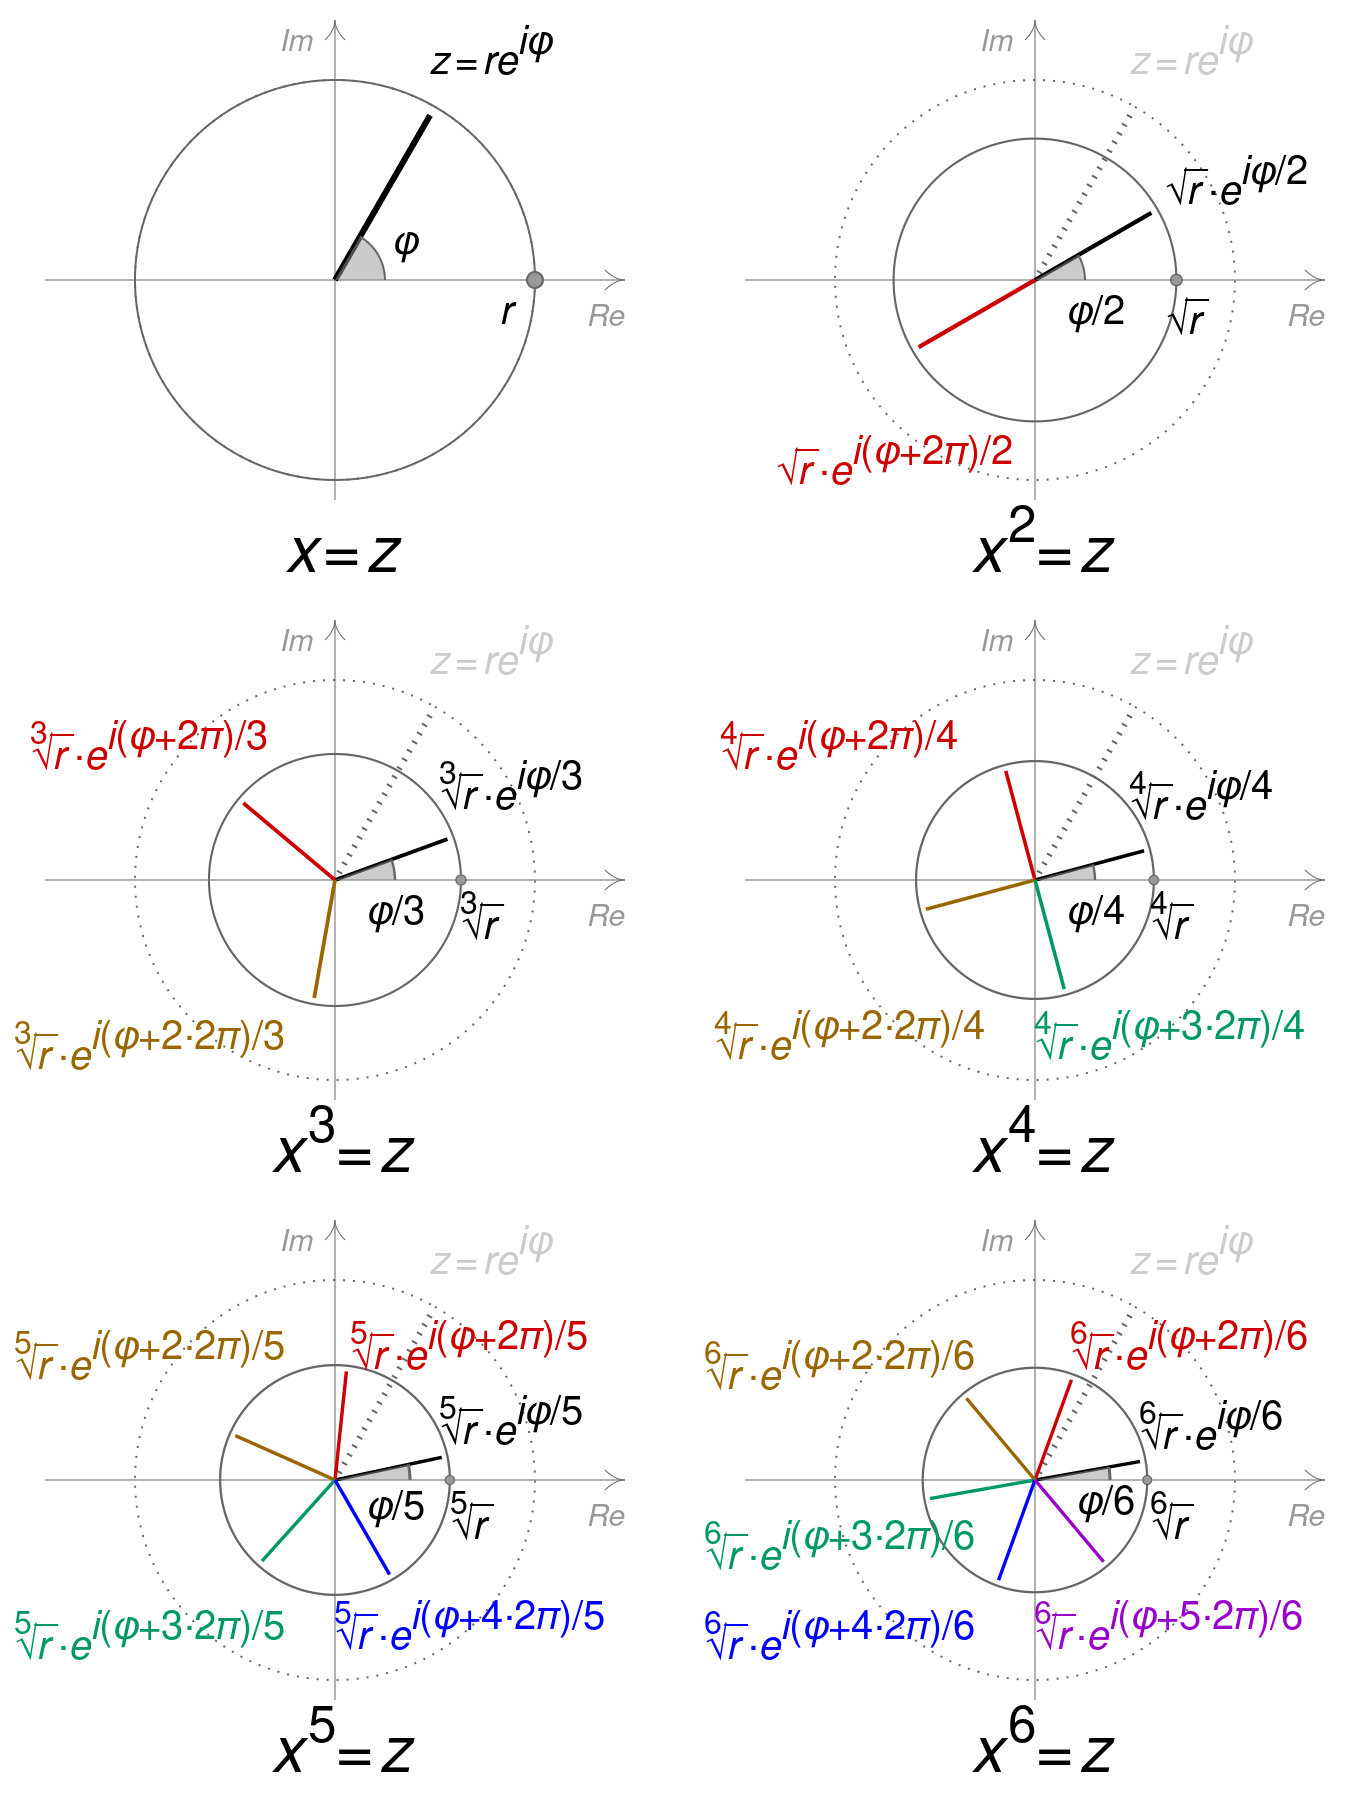
\includegraphics[width=0.5\textwidth]{img/Visualisation_complex_number_roots.png}
\end{figure}

\begin{property}
    \begin{enumerate}
        \item The \( n \)-th roots of unity form a \underline{cyclic group} under multiplication, 
            with \( \omega = \exp{\frac{2\pi i}{n}} \) as a generator.
    \end{enumerate}
\end{property}

\begin{proposition}{Formulas for Sums and Differences of Powers}
    For \(n \in \mathbb{N^+}\) and \(n\) being odd:
    \[
    a^n + b^n = (a+b)\big(a^{n-1}b^0 - a^{n-2}b^1 + a^{n-3}b^2 - \cdots - a^1b^{n-2} + a^0b^{n-1}\big).
    \]
    When \(n\) is even, there is no general formula for the \(n\)-th power sum.

    For \(n \in \mathbb{N^+}\):
    \[
    a^n - b^n = (a-b)\big(a^{n-1}b^0 + a^{n-2}b^1 + a^{n-3}b^2 + \cdots + a^0b^{n-1}\big).
    \]

    Commonly used special cases:
    \[
    a^2 - b^2 = (a+b)(a-b).
    \]
    \[
    a^3 + b^3 = (a+b)(a^2 - ab + b^2), \quad a^3 - b^3 = (a-b)(a^2 + ab + b^2).
    \]
    \[
    \begin{aligned}
    a^4 - b^4 &= (a^2 + b^2)(a^2 - b^2) = (a^2 + b^2)(a+b)(a-b), \\
    &= (a-b)(a^3 + a^2b + ab^2 + b^3).
    \end{aligned}
    \]
    When \(b=1\),
    \[
    x^n + 1 = (x+1)\big(x^{n-1} - x^{n-2} + x^{n-3} - \cdots + x - 1\big), \quad n \in \mathbb{N^+}, \, n \text{ is odd}.
    \]
    \[
    x^n - 1 = (x-1)\big(x^{n-1} + x^{n-2} + x^{n-3} + \cdots + x + 1\big), \quad n \in \mathbb{N^+}.
    \]
\end{proposition}






\chapter{Integral Valued Polynomials}



\section{Lagrange Interpolation Polynomial}

\chapter{Multivariate Polynomial}
\section{Symmetric Polynomial}
\begin{definition}{Symmetric Polynomial}
    A polynomial \( f(x_1, x_2, \ldots, x_n) \) in \( n \) variables is called a \textbf{symmetric polynomial} 
    if it remains unchanged under any permutation of its variables. 
    In other words, for any permutation \( \sigma \) of the set \( \{1, 2, \ldots, n\} \),
    the following holds:
    \[
    f(x_{\sigma(1)}, x_{\sigma(2)}, \ldots, x_{\sigma(n)}) = f(x_1, x_2, \ldots, x_n).
    \]
\end{definition}
Some common symmetric polynomials include:
\begin{description}
    \item[Elementary Symmetric Polynomials:] 
        \[
        e_k(x_1, x_2, \ldots, x_n) = \sum_{1 \leq i_1 < i_2 < \cdots < i_k \leq n} x_{i_1} x_{i_2} \cdots x_{i_k}, 
        \quad k = 1, 2, \ldots, n.
        \]
        That is,
        \begin{align*}
            &e_{0} = 1, \\
            &e_{1} = x_{1} + x_{2} + \cdots + x_{n}, \\
            &e_{2} = \sum_{1 \leq i < j \leq n} x_{i} x_{j}, \\
            &\vdots \\
            &e_{n} = x_{1} x_{2} \cdots x_{n}, \\
            &e_{k} = 0, \quad k > n.
        \end{align*}
    \item[Power Sum Symmetric Polynomials:] 
        \[
        p_k(x_1, x_2, \ldots, x_n) = x_1^k + x_2^k + \cdots + x_n^k, 
        \quad k = 1, 2, \ldots.
        \]
    \item[Complete Homogeneous Symmetric Polynomials:] 
        \[
        h_k(x_1, x_2, \ldots, x_n) = \sum_{i_1 + i_2 + \cdots + i_n = k} x_1^{i_1} x_2^{i_2} \cdots x_n^{i_n}, 
        \quad k = 1, 2, \ldots.
        \]
\end{description}



\begin{theorem}{Newton's Identities}
    For \( k \geq 1 \), the following relations hold between the elementary symmetric polynomials \( e_k \) 
    and the power sum symmetric polynomials \( p_k \):
    \[
    k e_k = \sum_{i=1}^{k} (-1)^{i-1} e_{k-i} p_i,
    \]
    where \( e_0 = 1 \) and \( e_k = 0 \) for \( k > n \).
\end{theorem}


\begin{thebibliography}{99}
\bibitem{en1} 南秀全, 黄振国. \emph{多项式理论}. 哈尔滨工业大学出版社, 2016.
\bibitem{en2} Author2, Title2, Journal2, Year2. \emph{ This is another example of a reference.}
\end{thebibliography}

\end{document}